%\vspace*{-15pt}
\section{Introduction}

%%AR: Rewriting based on structure we discussed in this doc: https://docs.google.com/document/d/1U5ZrJhdUCv2GBA6POek6pyLQSaqGmO1B-kTMI680pYU/edit

Offline reinforcement learning (offline RL)~\citep{LangeGR12, levine2020offline} refers to the setting where policies are trained using static, previously collected datasets. This presents an attractive paradigm for data reuse and safe policy learning in many applications, such as healthcare~\cite{Wang2018SupervisedRL}, autonomous driving~\cite{Yu2020BDD100KAD}, robotics~\cite{kalashnikov2018scalable, Rafailov2020LOMPO}, and personalized recommendation systems~\cite{SwaminathanJ15}. Recent studies have observed that direct use of RL algorithms originally developed for the online or interactive paradigm leads to poor results in the offline RL setting~\cite{fujimoto2018off, kumar2019stabilizing, kidambi2020morel}. This is primarily attributed to the distribution shift that arises over the course of learning between the offline dataset and the learned policy. Thus, development of algorithms specialized for offline RL is of paramount importance to benefit from the offline datasets available in the aforementioned application domains. In this work, we develop a new model-based offline RL algorithm that enjoys strong theoretical guarantees, while also matching or improving over state-of-the-art methods in offline RL benchmarks.

\begin{figure}[t!]
    \centering
    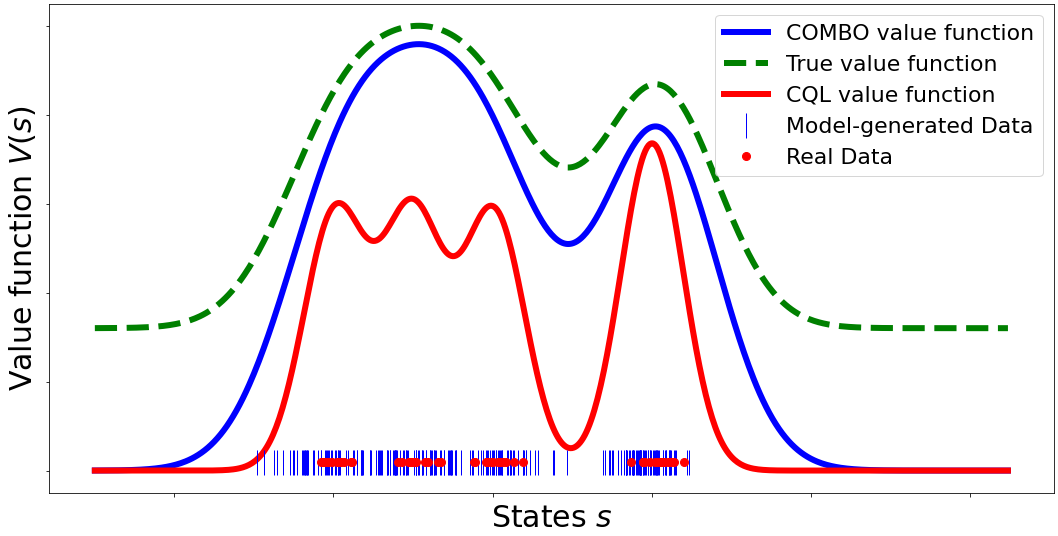
\includegraphics[width=0.45\textwidth]{teaser_combo.png}
    \vspace*{-0.5cm}
    \caption{COMBO learns a conservative value function by utilizing both the offline dataset as well as simulated data from the model. Crucially, COMBO does not require uncertainty quantification, and the value function learned by COMBO is a tighter lower-bound of the true value compared to CQL. This enables COMBO to steer the agent towards higher value states compared to CQL, which may steer towards sub-optimal states as illustrated in the figure.}
    \vspace*{-0.6cm}
    \label{fig:teaser}
\end{figure}

One paradigm for algorithm design in offline RL is to incorporate conservatism or regularization to the learning algorithm.
%This has led to the development of a number of recent algorithms which extend standard RL algorithms by incorporating various forms of conservatism to regularize the learning agent towards the offline dataset. 
Model-free offline RL algorithms~\cite{fujimoto2018addressing, kumar2019stabilizing, wu2019behavior,jaques2019way,kumar2020conservative}
%%SL.1.31: There are offline RL/batch RL algorithms going back decades (e.g., the Lange/Riedmiller survey). Reviewers who are well-versed in RL will roll their eyes a bit at the preceding statement.
directly incorporate conservatism into the policy or value function training
%%SL.1.31: the only one of the methods above that actually does this is kumar2020conservative, the rest all employ policy constraints of some sort and don't do anything to the value function explicitly (except indirectly due to the change in the policy)
%%AR: addressed by adding "policy or value training" -- the point to get across is that there are no models involved.
and do not require learning a dynamics model. 
%%CF: I removed the part about being more scalable. There are pretty scalable MBRL methods
However, model-free algorithms learn only on the states in the offline dataset, which can lead to overly conservative algorithms.
%%SL.1.31: I'm not sure this claim is really setting us up for success -- claiming gneeralization *outside the support* of the data seems like it's just impossible
%%AR: in the worst case, yes, but the hope is to gain in cases where generalization is possible (e.g. model bias is small). Solving novel tasks in MOPO is an example I think.
In contrast, model-based algorithms~\cite{kidambi2020morel, yu2020mopo} learn a pessimistic dynamics model, which in turn induces a conservative estimate of the value function. By generating data, model-based algorithms can achieve better generalization and e.g. have demonstrated the ability to solve new tasks using the offline dataset~\cite{yu2020mopo}.
However, such algorithms rely crucially on uncertainty quantification of the learned dynamics model to incorporate conservatism, which can be difficult or unreliable for complex datasets or deep network models.
Furthermore, these methods do not adapt the uncertainty estimates as the policy and value function change over the course of learning.
%%SL.1.31: The significance of this is not entirely clear (but I agree this is a true statement, and it's a nice observation, just that most readers won't get why this is important without more explanation)
In this work, our goal is to develop a new algorithm that retains the benefits of model-based algorithms while removing the reliance on uncertainty estimation, which we argue is not necessary for offline RL.

Our main contribution is the development of conservative offline model-based policy optimization (COMBO), a new model-based algorithm for offline RL. COMBO
learns a dynamics model using the offline dataset. Subsequently, it employs an actor-critic
method where the value function is learned using both the offline dataset as well as synthetically generated data from the model, similar to Dyna~\cite{sutton1991dyna}. However, in contrast to Dyna, COMBO learns a conservative critic function
by penalizing the value function in state-action tuples that are not in the support of the offline dataset, obtained by simulating the learned model. 
%
We theoretically show that for any policy, the Q-function learned with COMBO is a lower bound of the true Q-function, making it a good surrogate for policy optimization.
While the approach of optimizing a performance lower-bound is similar in spirit to prior model-based algorithms~\cite{kidambi2020morel, yu2020mopo},
COMBO crucially does not require uncertainty quantification.
%, making it easier to implement and more broadly applicable. 
In addition, we show theoretically that the Q-function learned by COMBO represents a tighter lower bound of the true Q-function when the model bias is low compared to prior model-free algorithms like CQL~\cite{kumar2020conservative}.
Thus, as a consequence of optimizing a tighter lower bound, COMBO has the potential to learn higher rewarding policies compared to prior model-free algorithms. This is illustrated through an example in Figure~\ref{fig:teaser}.
%%Ak.1.30: we say "overly conservative" at a bunch of places, but no where we mention the reason for that. Atleast we should make it clear that it is an empirical phenomenon and it intuitively happens because of controlling for state-distribution shift oonly via action distribution shift.
%%SL.1.31: definitely agreed, we need to better explain what this "overly conservative" thing actually means
%%AR: Addressed by rephrasing the claim.
Finally, in our experiments, we find that COMBO matches or exceeds the state-of-the-art results in commonly studied benchmark tasks for offline RL. Specifically, COMBO achieves the highest score in $9$ out of $12$ continuous control domains we consider from the D4RL~\cite{fu2020d4rl} benchmark suite, while the next best algorithm achieves the highest score in only $3$ out of the $12$ domains. We also show that COMBO achieves the best performance in tasks that require out-of-distribution generalization and outperforms previous latent-space offline model-based RL methods in the image-based robotic manipulation task.%%CF: Need to also mention the generalization results and the vision results!
%%TY.2.3: added a sentence on the generalization and vision results. Rafael, feel free to also add the vision-based locomotion task to the sentence if we are going to include the walker results. 
